\documentclass{book} %[a4paper,10pt]{article}
%\documentclass[a4paper,10pt]{scrartcl}

\usepackage[a6paper]{geometry}

%\usepackage{unit}
%\usepackage{gensymb}
\usepackage[utf8]{inputenc}
%\usepackage[textwidth=20cm]{geometry}
\usepackage{microtype}

\usepackage{pifont,mdframed}

\usepackage{colortbl,xcolor,array}
\usepackage{tabularx}

\usepackage{graphicx}
\graphicspath{ {images/} }

\definecolor{warningbackground}{HTML}{FFEB3B}
\definecolor{hintbackground}{HTML}{03A9F4}

\title{BlinkenHeart}
\author{FabLab Neuenstadt}
\date{20.07.2017}

\pdfinfo{%
  /Title    (BlinkenHeart)
  /Author   (FabLab Neuenstadt)
  /Creator  ()
  /Producer ()
  /Subject  (BlinkenHeart)
  /Keywords ()
}
	
\newcommand{\alertwarningbox}[1]{
\begin{center}
	\begin{tabularx}{\linewidth}{
			>{\columncolor{warningbackground}}c
			>{\columncolor{warningbackground}}X}
		\raisebox{\dimexpr2\baselineskip-\height/2-\tabcolsep}
		{
\includegraphics[width=1cm]{icons/001-warning}}&
		\raisebox{\tabcolsep}{\strut}\textbf{WICHTIG:} #1\raisebox{-\tabcolsep}{\strut}
	\end{tabularx}
\end{center}
}

\newcommand{\hintbox}[1]{
\begin{center}
	\begin{tabularx}{\linewidth}{
			>{\columncolor{hintbackground}}c
			>{\columncolor{hintbackground}}X}
		\raisebox{\dimexpr2\baselineskip-\height/2-\tabcolsep}
		{
\includegraphics[width=1cm]{icons/002-technology}}&
		\raisebox{\tabcolsep}{\strut}\textbf{TIPP:} #1\raisebox{-\tabcolsep}{\strut}
	\end{tabularx}
\end{center}
}


\begin{document}
\maketitle

\newpage
\section{Sicherheitshinweise}
Nach dem Löten musst du dir deine Hände gründlich mit Seife
waschen. Lötzinn ist nicht gesund und sollte nicht in die Nähe von
Essen kommen. Essen und Trinken solltest du beim Löten vermeiden!
\begin{center}
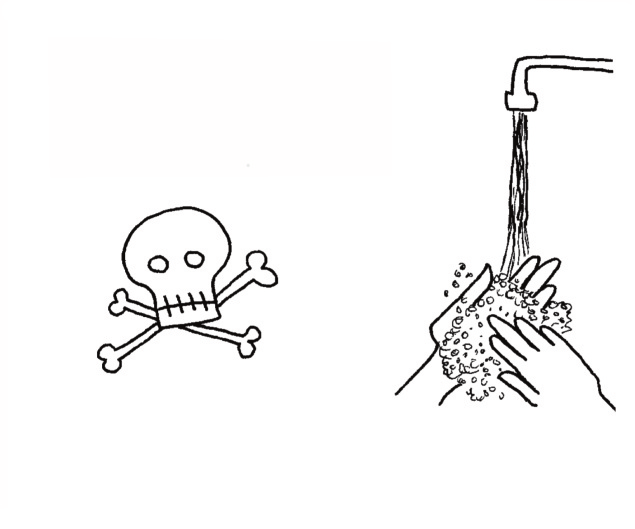
\includegraphics[width=5cm]{-000}
\end{center}

\newpage
\section{Löten lernen}
Zum Löten benötigst du einen Lötkolben, der auf eine Temperatur
zwischen 310$^\circ$C und 350$^\circ$C eingestellt werden muss. Bei dieser
Temperatur wird das Lötzinn flüssig und verbindet dein Bauteil mit der
Platine. Bei so viel Hitze kannst du dich und andere schnell verletzen.
Stelle deswegen den Lötkolben immer in die Halterung, wenn du ihn
gerade nicht benötigst.
\begin{center}
	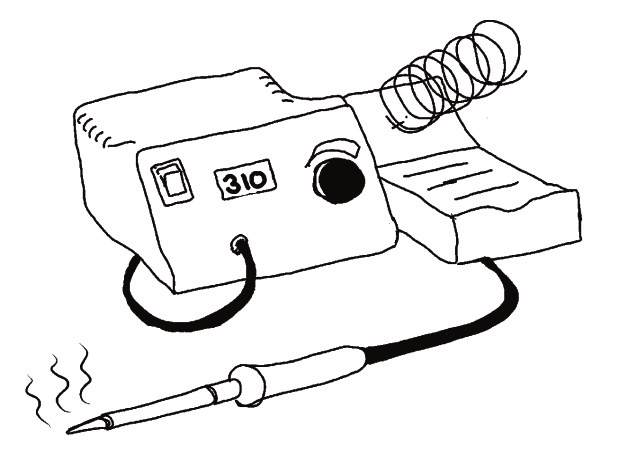
\includegraphics[width=5cm]{-002}
\end{center}

\section{bedrahtete Bauteile löten}
Stecke das Bauteil an der passenden Stelle durch die Löcher in der
Platine. Das Bauteil muss auf der bedruckten Seite aufliegen. Sollte das
Bauteil rausfallen, biege die Beinchen leicht zur Seite.
Nun lötest du nacheinander die Beinchen des Bauteils. Heize dazu
gleichzeitig das Beinchen des Bauteils und die Platine auf. Führe dann
seitlich etwas Lötzinn hinzu, bis sich ein kleiner Hügel Lötzinn bildet,
der das Loch vollständig bedeckt.
\begin{center}
	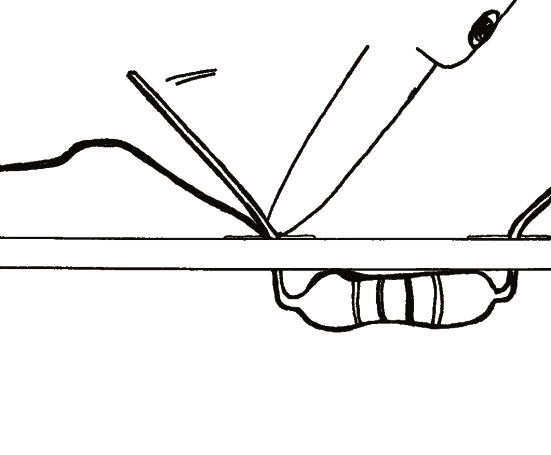
\includegraphics[width=5cm]{-004}
\end{center}

Die Lötstelle sollte ungefähr wie auf dem folgenden Bild aussehen.
Überflüssiges Lötzinn kannst du mit der Lötspitze an dem Drahtbeinchen
nach oben ziehen. Mit etwas Übung werden deine Lötstellen
immer besser!
\begin{center}
	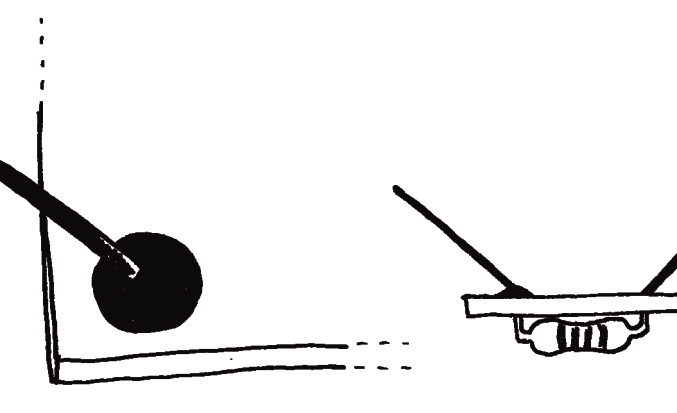
\includegraphics[width=5cm]{-006}
\end{center}

\section{SMD Bauteile löten}
SMD Bauteile sind Bauteile, die du auf der Oberfläche der Platine an so
genannte "Lötpads" anlötest. Lötpads sind Flächen auf der Platine, die
Lötzinn annehmen. Um ein SMD Bauteil anzulöten, erhitzt du die Platine
zunächst an den quadratischen oder rechteckigen Flächen, die wir
"Pad" nennen. Gib auf eine Seite eines Pad-Paares etwas Lötzinn bis
sich ein kleiner Berg Lötzinn gebildet hat. Es ist wichtig, dass immer nur
ein Pad mit Lötzinn bedeckt wird, sonst wird das Löten sehr schwierig!
\begin{center}
	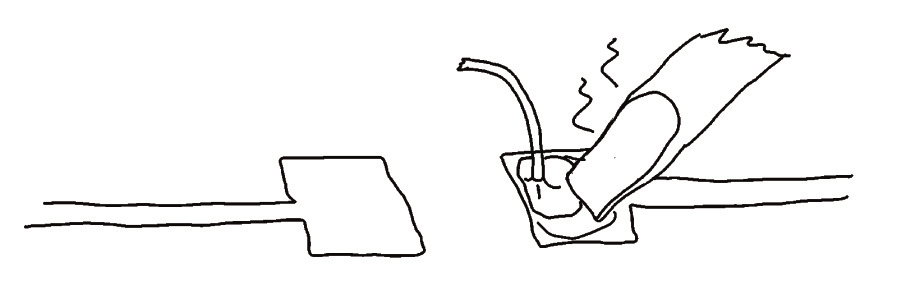
\includegraphics[width=5cm]{-010}
\end{center}

Halte nun den Lötkolben an das mit Lot bedeckte Pad und greife das
Bauteil gleichzeitig mit einer Pinzette. Schiebe das Bauteil mit einer
Seite in das flüssige Lot, so dass es mittig zwischen den beiden Pads
sitzt. Entferne nun den Lötkolben und halte das Bauteil solange fest, bis
das Lötzinn wieder fest geworden ist.
\begin{center}
	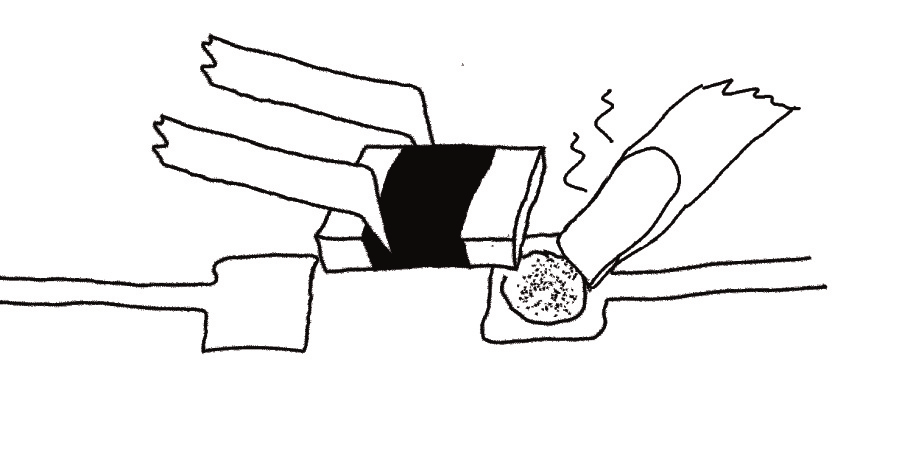
\includegraphics[width=5cm]{-008}
\end{center}

Um die andere Seite des Bauteils festzulöten, erhitzt du das Pad und
die noch fehlende Seite des Bauteils. Während du die Stelle mit dem
Lötkolben erhitzt, führst du solange etwas Lötzinn hinzu, bis die
Lötstelle wie auf dem Bild aussieht. Versuche das Bauteil zügig zu
löten, damit die gegenüberliegende Lötstelle nicht wieder warm wird.
Zu hohe Temperaturen über längere Zeit können das Bauteil
beschädigen.
\begin{center}
	%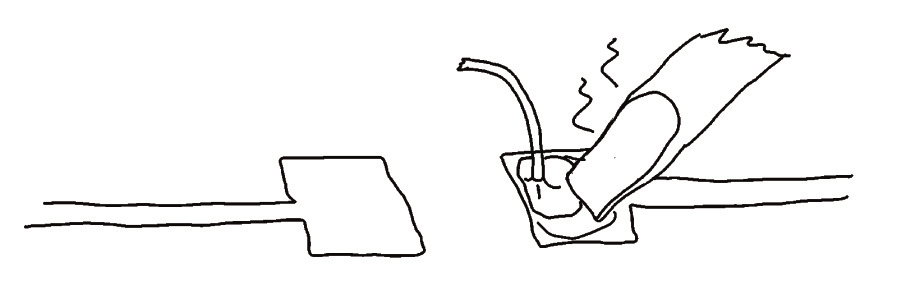
\includegraphics[width=5cm]{-010}
\end{center}

Deine Lötstellen sollten ungefähr so aussehen, wie auf dem Bild.
Die Pins der SMD Bauteile sollten seitlich komplett mit Lötzinn
benetzt sein. Wenn du die Platine nach dem Löten umdrehst,
dürfen die Bauteile nicht mehr abfallen.
\begin{center}
	%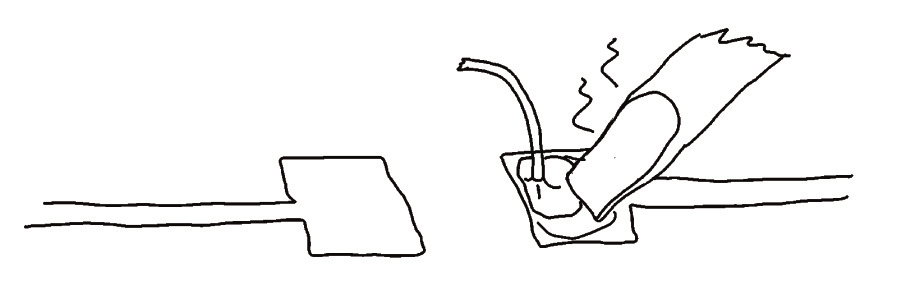
\includegraphics[width=5cm]{-010}
\end{center}

\section{SMD Bauteile mit vielen Kontakten löten}
Es gibt SMD Bauteile mit sehr vielen Kontakten, die wir häufig auch
Beinchen oder Pin nennen. Daher haben die Bauteile an der dafür
vorgesehenen Stelle auf der Platine auch sehr viele Pads. Mit der
richtigen Technik ist das allerdings für dich sicher kein Problem!
\begin{center}
	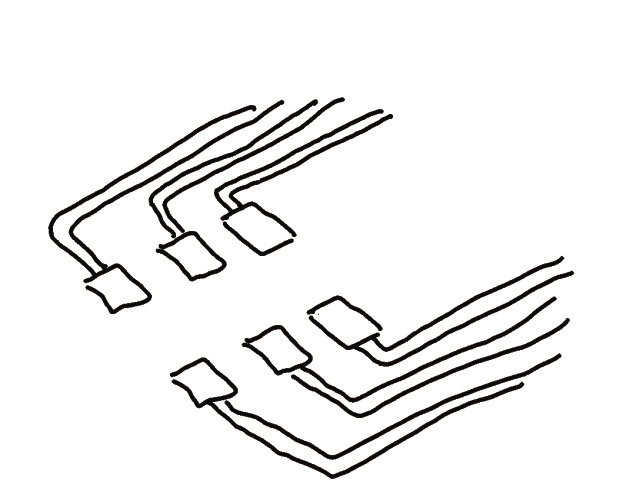
\includegraphics[width=5cm]{-012}
\end{center}

Zuerst suchst du dir ein Pad an einer Ecke des Bauteils aus und führst
etwas Lötzinn hinzu, bis ein kleiner Berg entsteht. Das Prinzip kennst du
schon von den SMD Bauteilen mit nur zwei Kontakten.

Anschließend setzt du das Bauteil mit einer Pinzette auf die Pads und
richtest alle Beinchen so aus, dass sie auf den Pads aufliegen. Halte
das Bauteil mit der Pinzette die ganze Zeit gut fest, damit es nicht
wegrutschen kann. Jedes Bauteil hat eine Markierung, z.B. einen Punkt,
oder eine Kerbe an der Seite, um dir die Ausrichtung anzuzeigen!
Wenn du Bauteile verdreht auflötest funktionieren sie nicht!

Nun erhitzt du den Pin mit dem Lötzinn, bis das Lötzinn geschmolzen
ist und den Pin umfließt. Nimm dann den Lötkolben weg und lasse das
Lötzinn wieder kalt werden. Wenn das Bauteil leicht verdreht ist, erhitze
den Pin wieder und drehe das Bauteil mit der Pinzette.
Jetzt lötest du den diagonal gegenüberliegenden Pin an, indem du Pin
und Lötpad erhitzt und etwas Lötzinn hinzufügst. Mache dann mit den
noch nicht gelöteten Pins weiter.
\begin{center}
	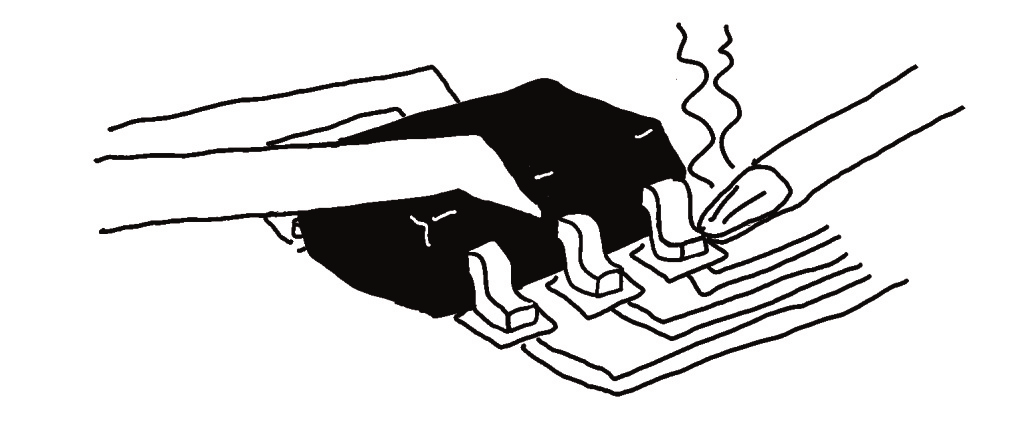
\includegraphics[width=5cm]{-016}
\end{center}

\newpage
\section{Löten}
Am besten du lötest die Bauteil-Gruppen in folgender Reihenfolge ein, da es so am einfachsten ist:
\begin{enumerate}
	\item Mikroprozessor
	\item Widerstände und Kondensatoren
	\item Schalter und Taster
	\item Leuchtdioden und Dioden
	\item Batteriehalter
\end{enumerate}
Die Gruppen sind auch nochmals in der Grafik mit der jeweiligen Nummer markiert.

\alertwarningbox{achte bei den Gruppen 1, 3, 4, 5 auf die korrekte Ausrichtung!
	Wenn diese Bauteile falsch herum eingelötet werden funktioniert das
	BlinkenHeart anschließend nicht.}
\hintbox{fange je Gruppe oben links an und löte dann jedes Bauteil einzeln im Uhrzeigersinn ein.
}

\begin{center}
	\includegraphics{pcb/solder_order}
\end{center}

\newpage
\section{Infos über die Bauteile}
\subsection{Prozessor}
Das als IC1 gekennzeichnete Bauteil enthält den Programmcode der BlinkenHeart und führt diesen aus. Es ist sozusagen das Gehirn der BlinkenHeart.

\hintbox{Der Programmcode kann aus unserem GitHub-Repository heruntergeladen und bei Interesse auch verändert werden. Besuche dafür einfach die Website github.com/FabLabNeuenstadt/BlinkenHeart oder scanne folgenden QR-Code:}
\begin{center}
	\includegraphics[width=3cm]{hw-repo-link}
\end{center}

\subsection{LEDs}
Die Bauteile die am Rand des BlinkenHeart sind
\textbf{L}ight \textbf{E}mitting \textbf{D}iodes.
Diese senden Licht aus sobald eine Spannung anliegt.
Jedoch nur wenn diese Spannung richtig herum anliegt.
Dies liegt daran, das LEDs die Eigenschaften einer Diode besitzt und
somit den Strom in einer Richtung blockiert.
Daher ist auch die Richtung der LEDs beim einlöten so wichtig.

\subsection{Widerstände}
Die unmittelbar in der Nähe des Prozessors platzierten Bauteile sind Widerstände. Diese dienen hier dazu den Strom zu begrenzen der durch die LEDs fließt da diese einen sehr geringen Eigenwiederstand haben. Wären diese Widerstände nicht vorhanden würden die LEDs nach kürzester Zeit kaputt gehen.

\subsection{Kondensator}
Das Bauteil C1, welches sich direkt unter dem untersten Widerstand befindet ist ein Kondensator. Es glättet die Eingangs-Spannung in dem Falle das die BlinkenHeart über USB mit Strom versorgt wird. Dies ist nur beim beschreiben der BlinkenHeart mit einem neuen Programm der Fall.

\newpage
\section{über BlinkenHeart}
\begin{center}
	
\includegraphics[width=5cm]{logo}
\end{center}
Die Bilder der Lötanleitung sind aus den Comics "Soldering is easy" von mightyohm.com und
"SMT soldering - it's easier than you think" von siliconfarmers.com entnommen und unter einer
Creative Commons Attribution Share-Alike Lizenz lizensiert.
Die Basis für diese Anleitung
und insbesondere der Teil für das Löten lernen wurde aus der Anleitung des CCC für die BlinkenRocket
von blinkenrocket.de entnommen.
Diese Anleitung und die BlinkenHeart Bilder sind ebenfalls unter dieser Lizenz lizensiert.
Die BlinkenHeart Platine ist unter der CERN Open-Hardware License Version 1.2 lizensiert, die Firmware steht unter der Lesser General
Public License Version 3.0 (LGPL V. 3.0) zur Verfügung.

Das Icon für die Hinweis-Box wurde von Chris Veigt erstellt und über www.flaticon.com bezogen.
Das Icon für die Tipp-Box wurde von Vectors Market erstellt und über www.flaticon.com bezogen.
\end{document}
